\documentclass{standalone}
\usepackage{tikz}

\begin{document}

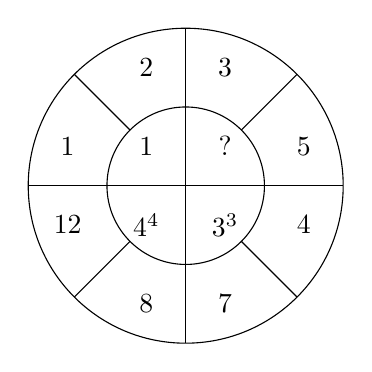
\begin{tikzpicture}
    \draw (0,0) circle (2cm);
    \draw (0,0) circle (1cm);

	\node at (0.5,0.5) {?};
    \node at (-0.5,0.5) {1};
    \node at (-0.5,-0.5) {$4^4$};
    \node at (0.5,-0.5) {$3^3$};

	\draw (0,-2)--(0,2);
	\draw (-2,0)--(2,0);

	\draw(0.707,0.707)--(1.414,1.414);
	\draw(-0.707,-0.707)--(-1.414,-1.414);
	\draw(-0.707,0.707)--(-1.414,1.414);
	\draw(0.707,-0.707)--(1.414,-1.414);

	\node at (0.5,1.5) {3};
    \node at (1.5,0.5) {5};
	\node at (-0.5,1.5) {2};
    \node at (-1.5,0.5) {1};
	\node at (-0.5,-1.5) {8};
    \node at (-1.5,-0.5) {12};
	\node at (0.5,-1.5) {7};
    \node at (1.5,-0.5) {4};
\end{tikzpicture}

\end{document}
